\documentclass[ignoreonframetext,unicode]{beamer}

\usepackage[utf8]{inputenc}
\usepackage[T1]{fontenc}
\usepackage[english,russian]{babel}
\usepackage{amsmath}
\usepackage{amsfonts}
\usepackage{amssymb}
\usepackage{graphicx,pgf}
\usepackage{multimedia}

\usetheme{Warsaw}

\useinnertheme{circles}   %внутренняя тема
%\useoutertheme{smoothbars}   %внешняя тема
\usecolortheme{seahorse}     %цветовая схема
%\usefonttheme{serif}    %шрифты
%\defbeamertemplate*{footline}{shadow theme}
%\setbeameroption{hide notes}

\graphicspath{{./style/}{./figures/}}

%номера слайдов
\newcommand*\oldmacro{}%
\let\oldmacro\insertshorttitle%
\renewcommand*\insertshorttitle{%
	\oldmacro\hfill%
	\insertframenumber\,/\,\inserttotalframenumber}
\RequirePackage{caption}
\DeclareCaptionLabelSeparator{defffis}{ }
\captionsetup{justification=centering,labelsep=defffis}

%\title{Курсовая работа}
%\subtitle{Численные схемы для аппроксимации неограниченных решений при моделировании обтекания профиля крыла в вихревых методах}
\title[Решение уравнения Рейнольдса]{Решение уравнения Рейнольдса в рамках теории газовой смазки методом конечных элементов}
\author[Пиневич В.\,Г.]{Докладчик: Пиневич В.\,Г.\and\\[0.5mm] Научный руководитель: Селиванов А.\,В.}

\institute[каф. Прикладная математика ФН-2]{группа ФН2-81Б}
\date{\today}
\titlegraphic{
\includegraphics[width=2cm]{logo.png}}
%\renewcommand{\vec}[1]{\text{\mathversion{bold}${#1}$}}


\begin{document}
	
	\begin{frame}[plain]
		\maketitle
		%\insertshortinstitute{Группа ФН2-41Б}
	\end{frame}

	\begin{frame}{Постановка задачи}
		\vspace*{-4mm}
		\begin{columns}
			\column{\textwidth}`
			\begin{block}{Уравнение Рейнольдса}
			 \[
				\frac{\partial}{\partial x} \left(h^3 \frac{\partial p}{\partial x} \right) + \frac{\partial}{\partial z} \left(h^3 \frac{\partial p}{\partial z} \right) = 6 \mu U \frac{\partial h}{\partial x}
			 \]
			\end{block}

\vspace*{-2mm}
		\begin{columns}
			\column{0.5\textwidth}
			\begin{block}{Граничные условия}
				$U$ --- скорость в направлении $x$,\\ 
				$p_{\text{в}}$ --- повышенное давление,\\ 
				$p_{\text{н}}$ --- пониженное давление
			\end{block}
		
			\column{0.5\textwidth}
			\begin{block}{Описание величин}
			$h = h(x)$ --- толщина слоя, \\
			$p = p(x, z)$ --- давление, \\
			$\mu$ --- коэффициент вязкости
			\end{block}
		\end{columns}

		\end{columns}
		
		\begin{figure}[!htbp]
			\centering
			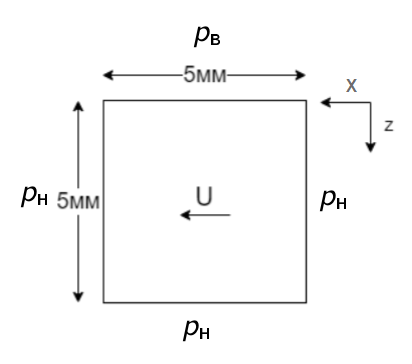
\includegraphics[width=0.4\textwidth]{taskGU}%
			\caption{Cхема области решения задачи}
			\vspace*{-2mm}
			\label{ser_graph}
		\end{figure}
		
	\end{frame}	

\begin{frame}{Решение уравнения Рейнольдса с помощью слабой формы Галеркина}
	
\begin{columns}
		
		\column{0.5\textwidth}
	\begin{block}{Функции формы}
		\[
			\begin{cases}
				N_1 = 1 - \frac{x}{l} - \frac{z}{h} + \frac{x  z}{l  h}, \\
				N_2 = \frac{x}{l} - \frac{x  z}{l  h}, \\
				N_3 = \frac{x  z}{l h}, \\
				N_4 = \frac{z}{h} - \frac{x  z}{l  h} \\
			\end{cases}
			\label{form-func}
		\]
		\end{block}
	
	\column{0.5\textwidth}
	\begin{block}{Входные данные}
	\[
		\begin{cases}
			h = 0.0001 \text{ м}, \\
			verticalLength = 0.005 \text{ м}, \\
			horizontalLength = 0.005 \text{ м}, \\
			\mu = 8.90 * 10^{-4} \text{ Па}*\text{с}, \\
			U = 10 \text{ м/c}, \\
			p_{\text{н}} = 100 \text{ кПа}, \\
			p_{\text{в}} = 150 \text{ кПа} \\
		\end{cases}	
	\]
\end{block}
\end{columns}

\begin{block}{Аппроксимирующая функция}
	\[
	\phi = c_0 N_1 + c_1 N_2 + c_2 N_3 + c_3 N_4
	\]
\end{block}
	
\end{frame}

\begin{frame}{Решение на сетке 10 на 10}
	
	\begin{columns}
		
		\column{0.5\textwidth}
		\begin{figure}[!htbp]
			\center{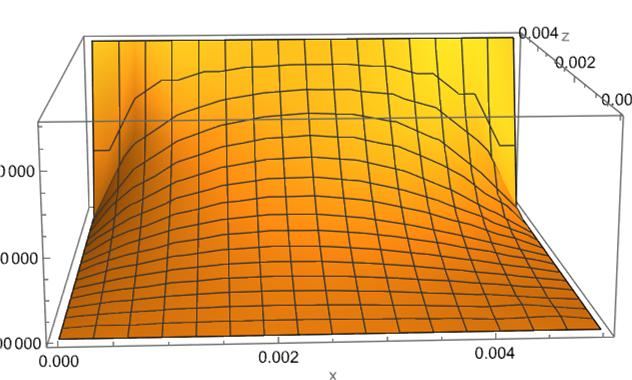
\includegraphics[width=\textwidth, height=0.5\textwidth]{10x10mesh.jpg}}
			\caption{График решения уравнения Рейнольдса для h = 0.0001 м на сетке 10 на 10 элементов}
			\label{10x10mesh}
		\end{figure}
		
		\column{0.5\textwidth}
		\begin{figure}[!htbp]
			\center{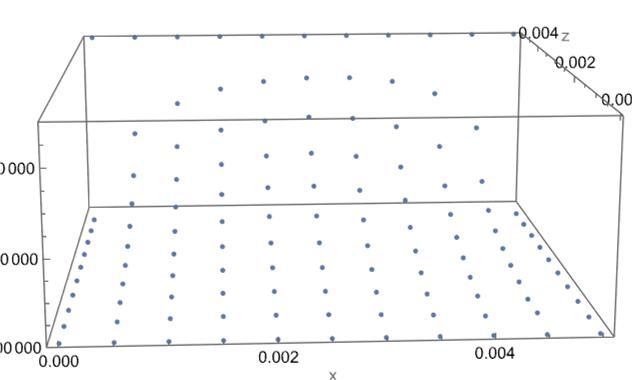
\includegraphics[width=\textwidth, height=0.5\textwidth]{10x10points.jpg}}
			\caption{График значений узлов решения уравнения Рейнольдса для h = 0.0001 м на сетке 10 на 10 элементов}
			\label{10x10points}
		\end{figure}
		
	\end{columns}
	
\end{frame}

\begin{frame}{Решение на сетке 20 на 20}
	
	\begin{columns}
		
		\column{0.5\textwidth}
		\begin{figure}[!htbp]
			\center{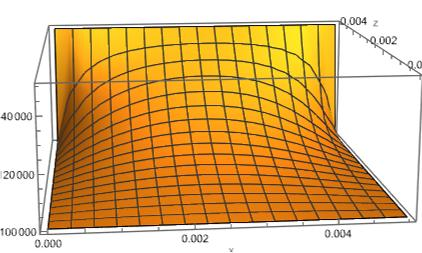
\includegraphics[width=\textwidth, height=0.5\textwidth]{20x20mesh.jpg}}
			\caption{График решения уравнения Рейнольдса для h = 0.0001 м на сетке 20 на 20 элементов}
			\label{5x5mesh}
		\end{figure}
		
		\column{0.5\textwidth}
		\begin{figure}[!htbp]
			\center{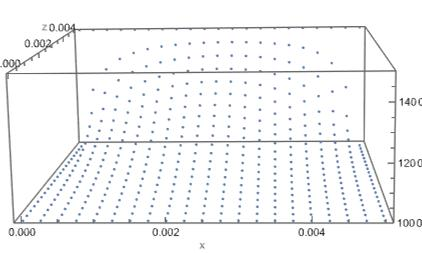
\includegraphics[width=\textwidth, height=0.5\textwidth]{20x20points.jpg}}
			\caption{График значений узлов решения уравнения Рейнольдса для h = 0.0001 м на сетке 20 на 20 элементов}
			\label{20x20points}
		\end{figure}
		
	\end{columns}
	
\end{frame}

\begin{frame}{Сравнение решения с Wolfram Mathematica}
	\vspace*{-4mm}
	\begin{figure}[!htbp]
		\center{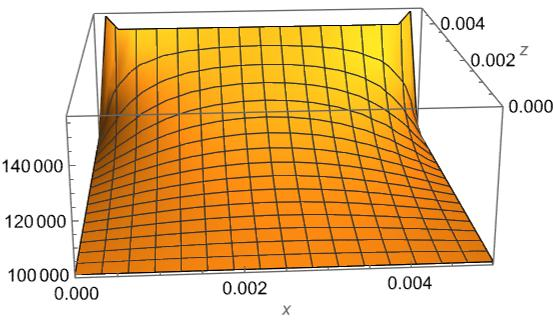
\includegraphics[width=\textwidth, height=0.4\textwidth]{exactSolutionConst.jpg}}
		\caption{График решения уравнения Рейнольдса для h = 0.0001 м полученный с помощью Wolfram Mathematica}
		\label{exactSolutionConst}
	\end{figure}

\begin{table}[!htbp]
	\begin{tabular}{|l|l|l|}
		\hline
		\multicolumn{1}{|c|}{Размерность сетки} & \multicolumn{1}{c|}{Разность, Па} & Погрешность, \% \\ \hline
		5 на 5                                  & 4612                              & 4.51            \\ \hline
		10 на 10                                & 1538                              & 1.38            \\ \hline
		20 на 20                                & 1290                              & 1.02            \\ \hline
	\end{tabular}
\end{table}
\end{frame}

\begin{frame}{Результаты}
	\begin{block}{Сделано}
	\begin{enumerate}	
		\item Создана программная реализация метода конечного элемента для решение уравнения Рейнольдса
		\item Полученные значения решения уравнения Рейнольдса были сравнены с результатами решения, полученного с помощью функции NDSolve в Wolfram Mathematica
	\end{enumerate}
	\end{block}	

	\begin{block}{Будет сделано}
	\begin{enumerate}	
		\item Получение базы аэродинамических усилий  для различных углов наклона и смещения верхней стенки на основе решения уравнения Рейнольдса
		\item Исследование динамического поведения пластинки с двумя степенями свободы, находящей под действием аэродинамических усилий со стороны потока жидкости
	\end{enumerate}
\end{block}	
\end{frame}	
\end{document} 